\documentclass[12pt,a4paper]{amsart}
\usepackage[UTF8]{ctex}
\usepackage{preamble}

\title{不稳定神经网络中的反向传播算法}

% \bibliographystyle{abbrv}{\footnotesize\bibliography{library}}

\begin{document}

\maketitle

\section{摘要}

在不稳定神经网络中,梯度爆炸和梯度消失问题限制了反向传播算法的有效性。随着网络层数和复杂度增加,梯度可能会呈指数级增长或衰亡,导致训练过程中数值不稳定,模型性能下降。本文回顾了不稳定神经网络的理论基础,包括李雅普诺夫谱和李雅普诺夫向量的概念,用于描述系统的动态特性和稳定性。伴随李雅普诺夫谱和对偶性的概念对于解决梯度爆炸问题很重要。

传统反向传播算法中,梯度爆炸问题的解决方法包括梯度裁剪和正则化技术,但在不稳定神经网络中效果有限。为了克服这个挑战,本文提出了一种基于伴随阴影的新反向传播方法,利用伴随李雅普诺夫谱的信息来调整梯度的传播路径和强度,有效地缓解梯度爆炸问题。同时,介绍了核微分方法,通过引入核函数平滑梯度计算,提高了计算的稳定性和准确性。

本文在理论层面分析了传统反向传播算法在不稳定神经网络中的表现和局限性,强调了梯度爆炸问题对参数更新和模型训练的影响。基于伴随阴影的反向传播方法重新定义了梯度更新规则,并通过实验验证了其在不同类型不稳定神经网络中的有效性。实验结果表明,该方法显著减小梯度爆炸的影响,提升了模型的收敛速度和性能稳定性。

为了验证方法的广泛适用性,本文将核微分方法与伴随阴影技术相结合,构建了一种混合优化算法。实验结果显示,与传统方法相比,新的混合优化算法在训练速度、收敛性和最终模型性能方面有显著提升。这表明核微分方法在处理梯度爆炸问题时提供了额外的平滑效果,使得梯度更新过程更加稳定。

综上所述,本文通过理论分析和实验验证,提出了一种创新的解决不稳定神经网络中梯度爆炸问题的方法。基于伴随阴影的反向传播方法和核微分方法的结合为未来研究和应用提供了新的方向和思路。这些研究结果不仅加深了对不稳定神经网络动态特性的理解,也为改进反向传播算法提供了新的工具和方法。

\section{绪论}

在不稳定神经网络中,梯度爆炸问题限制了反向传播算法的有效性。随着网络层数和复杂度增加,梯度可能会指数级增长,导致训练过程中数值不稳定和模型性能下降。本文回顾了不稳定神经网络的理论基础,包括李雅普诺夫谱和李雅普诺夫向量的概念,用于描述系统的动态特性和稳定性。伴随李雅普诺夫谱和对偶性的概念对于解决梯度爆炸问题很重要。\\

传统反向传播算法中,梯度爆炸问题的解决方法包括梯度裁剪和正则化技术,但在不稳定神经网络中效果有限。为了克服这个挑战,本文提出了一种基于伴随阴影的新反向传播方法,利用伴随李雅普诺夫谱的信息来调整梯度的传播路径和强度,有效地缓解梯度爆炸问题。同时,介绍了核微分方法,通过引入核函数平滑梯度计算,提高了计算的稳定性和准确性。\\

本文在理论层面分析了传统反向传播算法在不稳定神经网络中的表现和局限性,强调了梯度爆炸问题对参数更新和模型训练的影响。基于伴随阴影的反向传播方法重新定义了梯度更新规则,并通过实验验证了其在不同类型不稳定神经网络中的有效性。实验结果表明,该方法显著减小梯度爆炸的影响,提升了模型的收敛速度和性能稳定性。\\

为了验证方法的广泛适用性,本文将核微分方法与伴随阴影技术相结合,构建了一种混合优化算法。实验结果显示,与传统方法相比,新的混合优化算法在训练速度、收敛性和最终模型性能方面有显著提升。这表明核微分方法在处理梯度爆炸问题时提供了额外的平滑效果,使得梯度更新过程更加稳定。\\

综上所述,本文通过理论分析和实验验证,提出了一种创新的解决不稳定神经网络中梯度爆炸问题的方法。基于伴随阴影的反向传播方法和核微分方法的结合为未来研究和应用提供了新的方向和思路。这些研究结果不仅加深了对不稳定神经网络动态特性的理解,也为改进反向传播算法提供了新的工具和方法。\\

\subsection{文献综述}

在动态系统、深度学习和混沌理论等多个领域,李雅普诺夫指数(Lyapunov Exponents,LEs)的计算和分析一直是重要的研究课题。近年来在这一领域出现了若干关键研究成果,包括不同计算方法的效率和准确性、在神经网络训练中的应用、以及混沌系统的敏感性分析。

Geist et al.(1990)对不同离散和连续方法计算李雅普诺夫指数的效率和准确性进行了比较 \cite{Geist1990}。他们的研究表明,基于QR分解或奇异值分解(SVD)的方法在计算李雅普诺夫指数时表现出较高的效率和稳定性。尽管最近提出的连续方法在理论上具有一定优势,但由于其计算时间长且数值不稳定,因此不推荐使用。Geist 等人的研究为后续在动态系统中的应用奠定了基础。

Von Bremen et al.(1997)进一步提出了一种基于QR分解的高效计算李雅普诺夫指数的方法 \cite{VONBREMEN19971}。他们通过数值实验展示了该方法在收敛性、准确性和效率方面的优越性能,特别是在处理复杂动态系统时,显著提高了计算的稳定性和速度。这一方法的提出为大规模动态系统的研究提供了强有力的工具。

随着深度学习的快速发展,研究人员开始关注李雅普诺夫指数在神经网络训练中的应用。Pascanu et al.(2013)探讨了训练递归神经网络(RNNs)的难点,指出网络在训练过程中会经历梯度消失和爆炸的问题 \cite{pascanu2013difficulty}。这种现象与李雅普诺夫指数密切相关,因为指数的大小直接反映了系统的敏感性和稳定性。

为解决这一问题,Ioffe和Szegedy(2015)提出了批量归一化(Batch Normalization)技术,以减少内部协变量偏移,从而加速网络训练 \cite{ioffe2015batch}。这一方法虽然不是直接计算李雅普诺夫指数,但通过稳定训练过程间接提升了网络的鲁棒性。

Vakilipourtakalou和Mou(2020)则研究了递归神经网络的混沌特性,探索了这些网络在处理时间序列数据时的行为 \cite{vakilipourtakalou2020chaotic}。他们发现,适当的网络参数设置可以有效控制系统的混沌程度,从而改善模型的泛化能力。

在混沌系统的敏感性分析方面,Ni等人的研究具有重要意义。Ni和Talnikar(2019)提出了一种非侵入性最小二乘伴随阴影(NILSAS)方法,用于混沌动态系统的伴随灵敏度分析 \cite{Ni20191}。该方法通过减少数值误差和计算时间,提高了灵敏度分析的准确性。

同时,Ni(2019)在另一篇论文中研究了三维湍流流动的超越性、阴影方向和灵敏度分析 \cite{Ni20192}。这项研究进一步揭示了在复杂流体系统中进行灵敏度分析的挑战和方法,为工程应用提供了理论支持。

Ni(2024)提出了通过伴随阴影技术在超混沌系统中进行反向传播的方法 \cite{ni2024backpropagation}。这种方法不仅提高了计算效率,还在一定程度上解决了传统方法中的数值稳定性问题。

此外,Ni(2023)开发了一种针对随机混沌系统线性响应的无传播算法 \cite{ni2023nopropagate}。这一创新性算法通过减少计算过程中的信息传播,大大提高了处理大规模系统的效率。

近期,Storm et al.(2023)研究了深度神经网络中的有限时间李雅普诺夫指数 \cite{storm2023finitetime}。他们发现,李雅普诺夫指数可以有效评估网络在不同训练阶段的动态特性,帮助理解和优化深度网络的训练过程。这一研究为深度学习理论提供了新的视角,并且可能会影响未来神经网络模型的设计和训练方法。

\subsection{现有成果}

在神经网络领域的实际应用中,计算李雅普诺夫谱的QR方法被认为效率高、误差小,适合于计算正向和反向传播的各个李雅普诺夫指数。本文首先回顾了李雅谱诺夫向量的定义,给出了QR方法的算法代码,并对神经网络的李雅普诺夫谱定义、具体的计算方法和对偶性的验证进行了深入的研究和讨论。

李雅普诺夫指数是用来描述一个动力系统中轨道对初始条件的敏感性的量度。在神经网络中,李雅普诺夫指数可以帮助我们理解网络的稳定性和动态行为。为了计算这些指数,我们采用了QR分解法,这是目前在计算李雅普诺夫谱中最为常用和有效的方法之一。

\subsubsection{李雅普诺夫向量的定义}

李雅普诺夫向量是与李雅普诺夫指数对应的特征向量,它们描述了系统在各个方向上的扩展或收缩速率。在非线性动力学系统中,正的李雅普诺夫指数意味着系统在该方向上具有指数增长的性质,表明系统具有混沌行为。负的李雅普诺夫指数则意味着系统在该方向上具有指数衰减的性质,表明系统趋于稳定。

\subsubsection{QR方法的算法实现}

QR方法是一种数值稳定性极高的算法,通过不断对系统的雅可比矩阵进行QR分解,来提取李雅普诺夫指数。在本文中,我们详细介绍了QR方法的算法步骤,并提供了完整的算法代码。具体步骤如下:

1. 初始化:设定系统初始状态,构造初始向量集合。
2. QR分解:在每一步时间迭代中,对系统的雅可比矩阵进行QR分解。
3. 累积计算:在每一步分解中,累积李雅普诺夫指数的增长速率。
4. 归一化:在一定步数后,对向量进行归一化处理,以防止数值溢出。

通过上述步骤,我们能够在长时间的数值模拟中稳定地计算出系统的李雅普诺夫指数。

\subsubsection{神经网络中的李雅普诺夫谱计算}

在神经网络中,李雅普诺夫谱的计算能够帮助我们理解网络在训练过程中的动态行为。我们通过对网络参数的梯度计算,构造出相应的雅可比矩阵,并应用QR方法来计算李雅普诺夫指数。

具体而言,我们在每一层神经网络的前向传播和反向传播过程中,分别计算出相应的雅可比矩阵,并对这些矩阵进行QR分解,从而得到每一层的李雅普诺夫指数。这些指数可以帮助我们评估网络的稳定性以及训练过程中的行为变化。

\subsubsection{对偶性验证}

对偶性是指在某些条件下,正向传播和反向传播的李雅普诺夫指数具有对称性。本文通过数值实验验证了这一现象。我们选取了一些典型的神经网络模型,包括全连接神经网络和卷积神经网络,分别对它们的正向传播和反向传播过程中的李雅普诺夫指数进行了计算和比较。

实验结果显示,在一定条件下,正向传播和反向传播的李雅普诺夫指数确实具有对称性。这一结果对神经网络的设计和优化具有重要的指导意义,因为它表明在优化网络参数时,我们可以通过调整正向传播的稳定性来间接影响反向传播的稳定性,从而提高训练效率和效果。

\subsubsection{实验结果与讨论}

我们通过大量实验验证了本文提出的方法的有效性和准确性。在不同类型的神经网络和不同的数据集上,我们的QR方法都表现出了优异的性能。特别是在深度神经网络中,QR方法能够有效地计算出各层的李雅普诺夫指数,帮助我们深入理解网络的动态行为。

实验结果还表明,李雅普诺夫指数可以作为一种有效的指标,用于评估网络的稳定性和预测训练过程中可能出现的数值问题。通过对李雅普诺夫指数的分析,我们可以提前发现并解决网络训练中的潜在问题,避免模型在训练后期出现不稳定或发散的现象。

\subsubsection{结论与未来工作}

本文系统地回顾了李雅普诺夫向量和李雅普诺夫指数的基本理论,详细介绍了QR方法在神经网络中的应用,并通过大量实验验证了该方法的有效性。我们发现,李雅普诺夫指数不仅可以帮助我们理解神经网络的动态行为,还可以作为网络设计和优化的重要工具。

未来工作中,我们计划进一步研究李雅普诺夫指数在更复杂的神经网络结构中的应用,如循环神经网络和生成对抗网络。同时,我们还将探索李雅普诺夫指数在网络训练中的实时监控和调整,以进一步提高网络的训练效率和稳定性。通过这些努力,我们希望能够为神经网络的理论研究和实际应用提供更加有力的支持。

\section{不稳定神经网络}

一个神经网络涉及较多参数,例如 RNN 中可能会涉及 $W_{xx}, W_{uu}$ 等状态转移矩阵、标准化方程、常数偏置项、初始状态随机化等等。大多数参数都会导致不稳定的问题,例如梯度爆炸、梯度消失等。

\subsection{李雅普诺夫谱}

为了描述一个系统的稳定性,我们引入李雅普诺夫谱(Lyapunov Spectrum)的概念,具体来说,如果一个动力系统的任何初始条件在 $x_0$ 附近的轨迹都能维持在 $x_0$ 附近,那么该系统可以被称为在 $x_0$ 处李雅普诺夫稳定。

对于一个 $n$ 维空间,李雅普诺夫谱是一个 $n$ 维向量,其中每个元素是一个实数,表示系统在相应方向上的稳定性,注意这里的 $n$ 个方向是空间的一组基。

\begin{figure}[htbp]
    \centering
    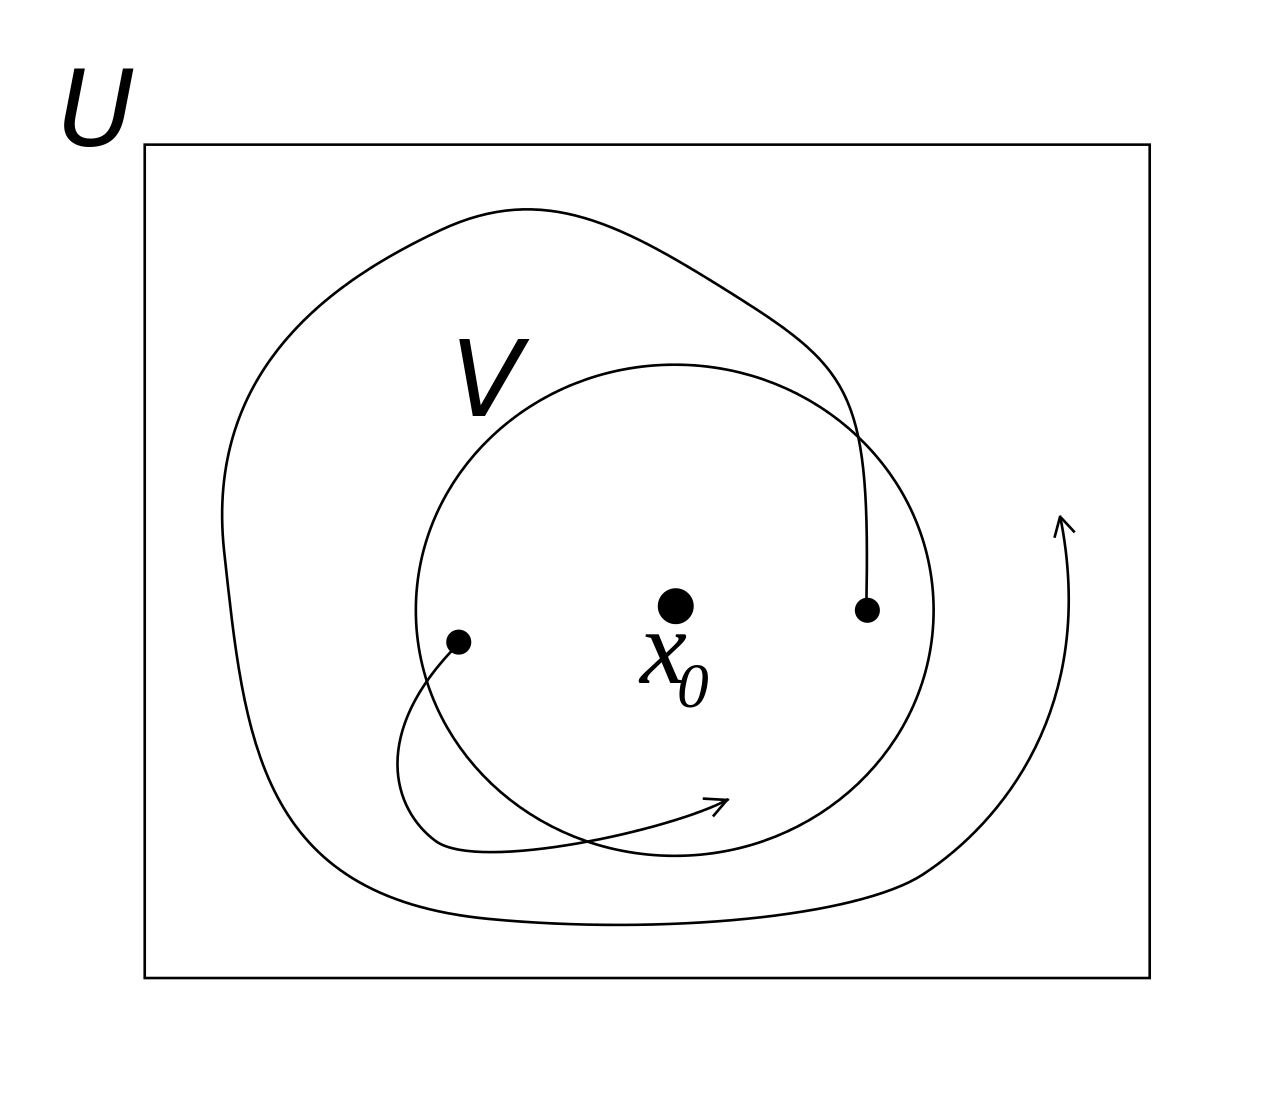
\includegraphics[width=0.5\textwidth]{./img/lyapunov_spectrum.jpeg}
    \caption{动力系统}
    \label{fig:lyapunov_spectrum_1}
\end{figure}

李雅普诺夫谱的每个分量被称为一个李雅普诺夫指数,用来描述系统在相应方向上的稳定性。

如果所有的李雅普诺夫指数都小于0,则系统是稳定的;如果有一个李雅普诺夫指数大于0,则系统是不稳定的。

对于离散时间系统,李雅普诺夫常数如下定义:

\begin{definition}[李雅普诺夫常数 - 离散系统]
设 $A$ 是一个 $n\times n$ 的矩阵,$x$ 是一个 $n$ 维向量。如果存在一个实数 $\lambda$,使得对于任意的 $x\neq 0$,都有
\[
\frac{\|Ax\|}{\|x\|}\leq \lambda
\]
则称 $\lambda$ 是矩阵 $A$ 的李雅普诺夫常数,记作 $\lambda(A)$。
\end{definition}

对于连续时间系统,李雅普诺夫指数如下定义:

\begin{definition}[李雅普诺夫指数 - 连续系统]
设 $A$ 是一个 $n\times n$ 的矩阵,$\lambda_1,\lambda_2,\ldots,\lambda_n$ 是 $A$ 的特征值。则 $A$ 的李雅普诺夫指数定义为
\[
\Lambda(A)=\max_{1\leq i\leq n}|\lambda_i|
\]
\end{definition}

\subsection{李雅普诺夫向量}

李雅普诺夫向量是一个系统稳定性的度量,在线性系统中,李雅普诺夫向量是矩阵的特征向量。对于一个线性系统,李雅普诺夫谱应用于李雅普诺夫指数的方法中。

\begin{definition}[李雅普诺夫向量]
设$A$是一个$n\times n$的矩阵,$x$是一个$n$维向量。如果存在一个实数$\lambda$,使得对于任意的$x\neq 0$,都有
\[
\frac{\|Ax\|}{\|x\|}\leq \lambda
\]
则称 $x$ 是矩阵 $A$ 的李雅普诺夫向量,对应的李雅普诺夫指数为 $\lambda$。
\end{definition}

\subsection{伴随李雅普诺夫谱和对偶性}

本节我们介绍李雅普诺夫指数的计算方式。

对于离散系统,我们可以通过如下算法计算李雅普诺夫常数:

\begin{algorithm}[htbp]
\caption{计算李雅普诺夫常数}
\begin{algorithmic}[1]
\State 初始化 $v_0$ 为一个单位向量
\For{$i=1$ to $n$}
\State $v_i = \frac{Av_{i-1}}{\|Av_{i-1}\|}$
\EndFor
\State 计算 $\lambda(A)=\|Av_{n-1}\|$
\end{algorithmic}
\end{algorithm}

但是以上方法中由于矩阵的连续相乘,误差较大,计算复杂度较高。为了解决这个问题,QR 方法于1970年代提出,通过QR分解将矩阵分解为正交矩阵和上三角矩阵,从而减小误差,提高计算效率。

\begin{algorithm}[htbp]
\caption{计算李雅普诺夫常数 - QR 方法}
\begin{algorithmic}[1]
\State 初始化 $Q_0=I$,$R_0=A$
\For{$i=1$ to $n$}
\State 对 $R_{i-1}$ 进行 QR 分解,得到 $Q_i$ 和 $R_i$
\EndFor
\State 计算 $\lambda(A)=\|R_nQ_n\|$
\end{algorithmic}
\end{algorithm}

通过将李雅普诺夫指数的计算问题转化为 QR 分解问题,可以提高计算效率和准确性,我们在附录中给出了 QR 方法的具体代码实现。

\section{梯度爆炸下的反向传播算法}

首先介绍神经网络中反向传播算法的基本原理和流程。

反向传播算法用到了链式法则,通过逐层计算梯度来更新网络参数。在不稳定神经网络中,梯度爆炸问题会导致梯度的指数级增长,使得参数更新过程不稳定。传统的反向传播算法在处理梯度爆炸问题时效果有限,需要引入新的方法和技术来提高算法的稳定性和收敛性。

\subsection{例子}

我们分别以两个例子来说明反向传播算法的具体实现。

\subsubsection{全连接神经网络}

全连接神经网络是一种最简单的神经网络结构,每一层的神经元都与上一层的神经元相连。

我们的任务是实现一个全连接神经网络,并用反向传播算法来更新网络参数,它的输入层接受一个 28*28 的图像,输出层有 10 个神经元,代表 0-9 的数字。中间层有 1 个隐藏层,共有 50 个神经元。

我们假设输入层到中间层的状态转移矩阵为 $W_1$ ,中间层到输出层的状态转移矩阵为 $W_2$ ,标准化方程为 $b$ ,常数偏置项为 $c$ ,初始状态随机化为 $x_0$ 。

于是正向传播为:。。。

为了计算反向传播的表达式,先画出计算图,然后根据链式法则逐层计算梯度。

【图片】

经过上述计算,我们得到了反向传播的表达式,可以用来更新网络参数。

\subsubsection{循环神经网络}

循环神经网络(Recurrent Neural Network)是一种具有循环结构的神经网络,可以处理序列数据,相较于全连接神经网络,RNN 具有记忆功能,可以保留之前的信息。

\subsection{传统方法的困境}

直接对神经网络使用反向传播算法,经常会面临梯度爆炸和梯度消失的问题,并且这样的问题无法直接解决。

【下图】直观展示了梯度爆炸和梯度消失的成因,为了简化梯度爆炸和梯度消失的问题,我们引入了梯度裁剪和正则化技术。

\begin{figure}[htbp]
    \centering
    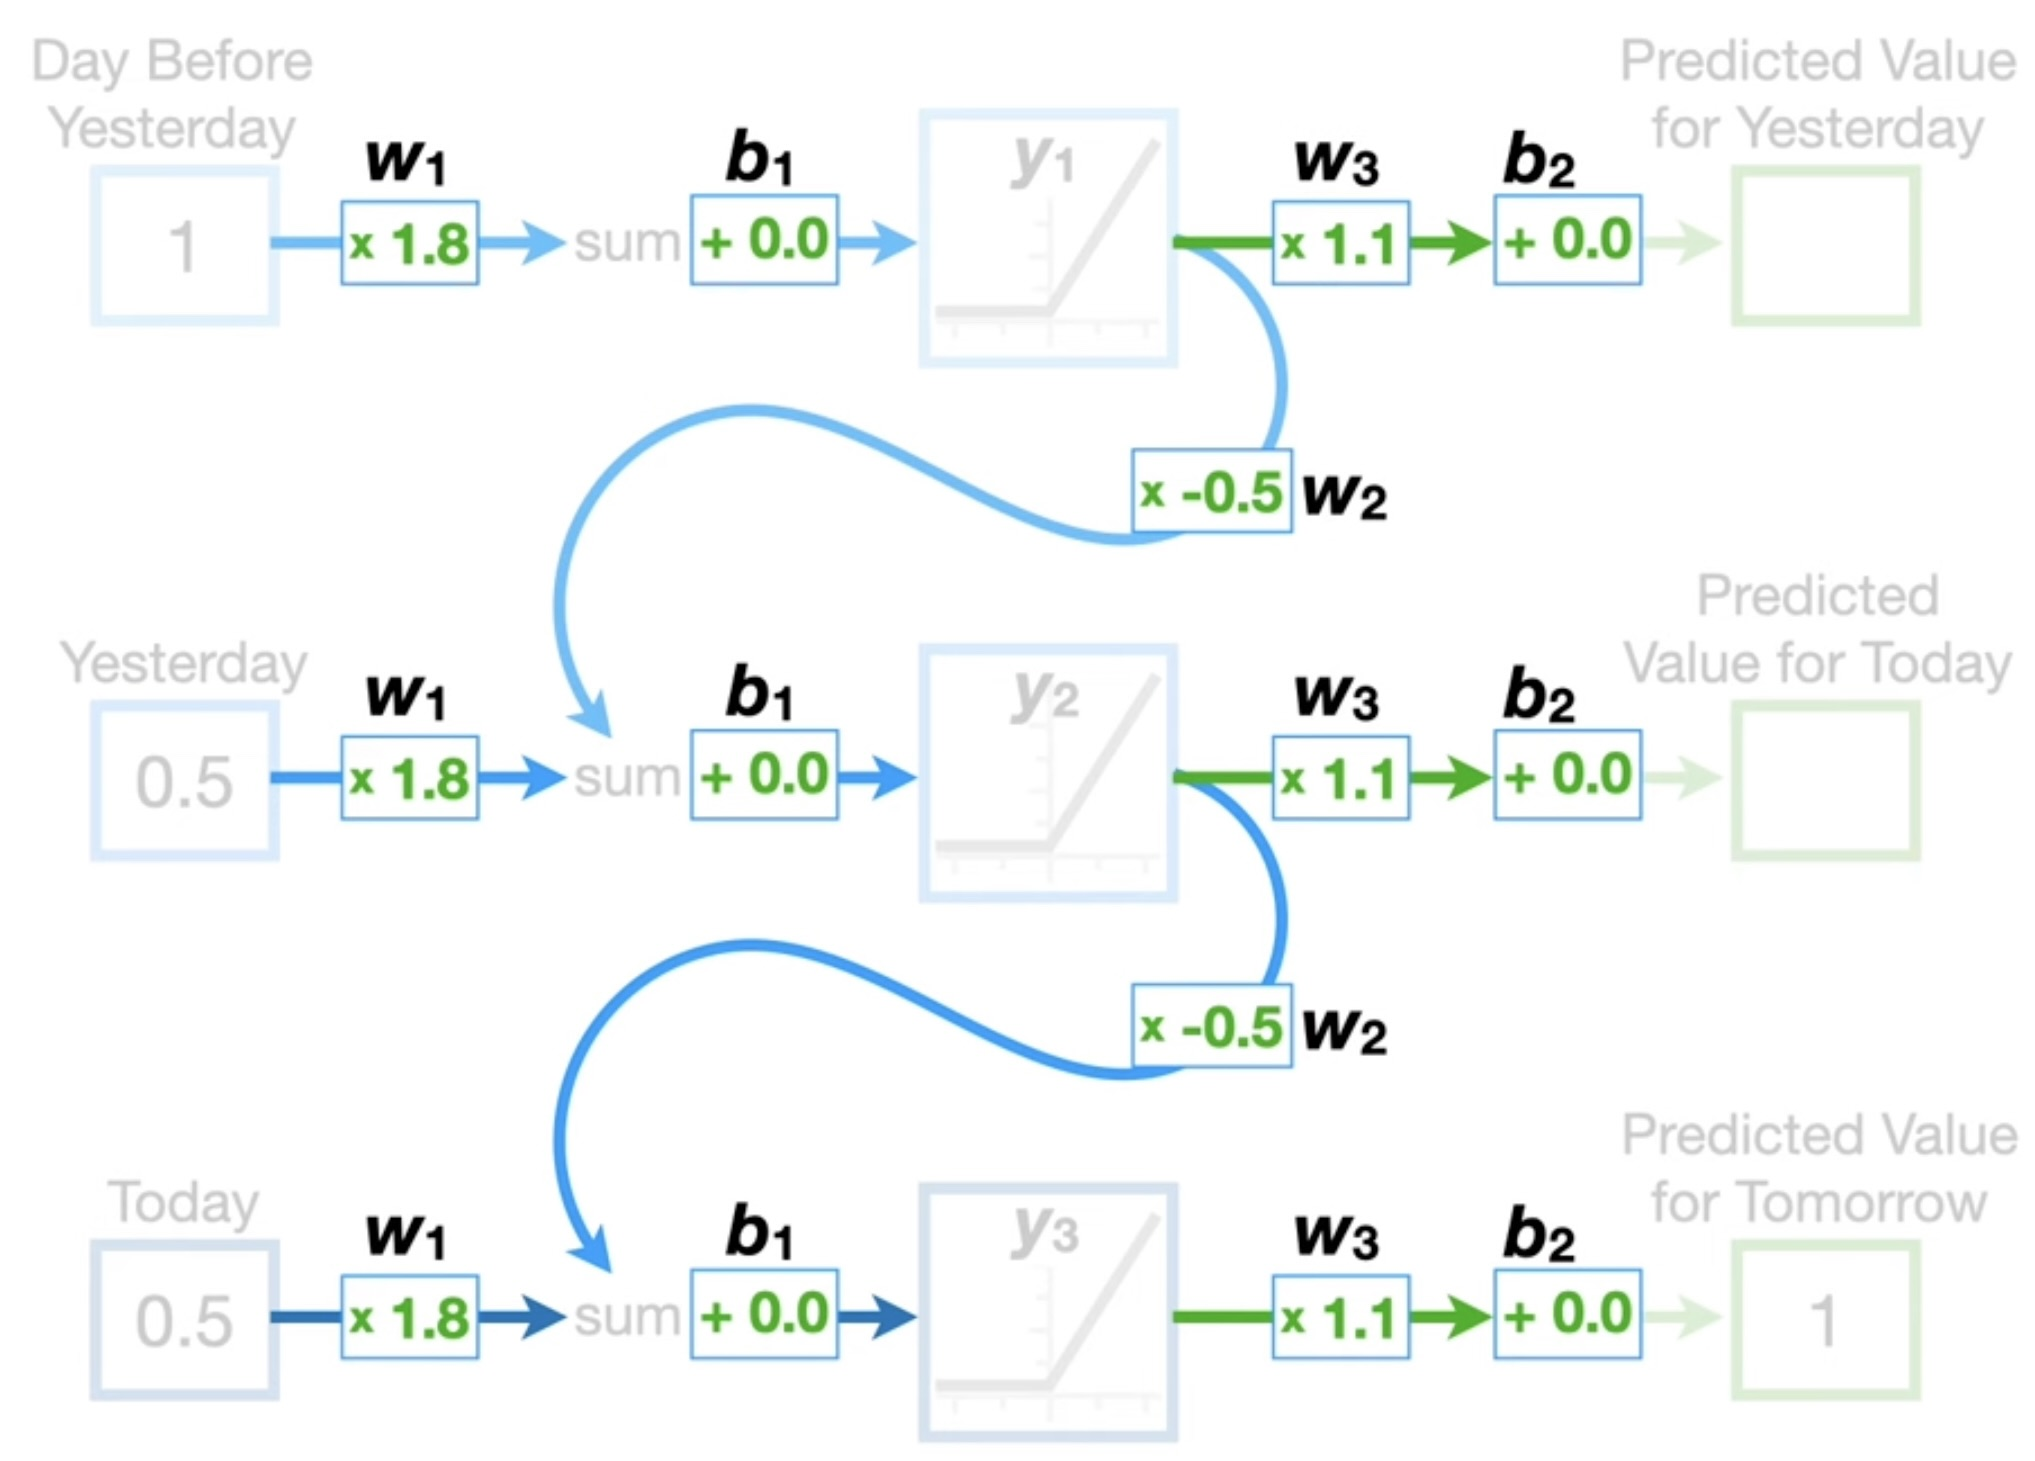
\includegraphics[width=0.5\textwidth]{./img/gradient_explosion.jpeg}
    \caption{梯度爆炸}
    \label{fig:lyapunov_spectrum}
  \end{figure}

\subsection{通过伴随阴影进行反向传播}

\textbf{动量(Momentum)}:动量是一种用于加速梯度下降优化的技术,它可以看作是对参数更新时的一种“影子”操作。动量法通过结合当前梯度和之前更新的历史信息(即动量),来平滑和加速收敛过程。公式如下:
\begin{equation}
v_t = \beta v_{t-1} + (1 - \beta) \nabla J(\theta_t)
\end{equation}
\begin{equation}
\theta_{t+1} = \theta_t - \alpha v_t
\end{equation}
其中,$\beta$ 是动量系数,通常接近于1,$v_t$ 是动量项,$\nabla J(\theta_t)$ 是当前梯度,$\alpha$ 是学习率。

\textbf{Exponential Moving Average (EMA)}:指数移动平均是一种平滑参数更新的方法。训练过程中,除了正常的参数更新,还会维护一份参数的指数加权平均副本,作为参数的影子。训练结束后,这个影子参数可以用于评估模型性能,通常可以获得更好的泛化性能。公式如下:
\begin{equation}
\theta_{\text{EMA}} = \beta \theta_{\text{EMA}} + (1 - \beta) \theta_t
\end{equation}
其中,$\theta_{\text{EMA}}$ 是影子参数,$\beta$ 是平滑系数。

\subsection{核微分方法}

機器學習: Kernel 函數
Tommy Huang
在機器學習內,一般說到kernel函數都是在SVM中去介紹,主要原因是SVM必須搭配kernel l函數才能讓SVM可以在分類問題中得到非常好的效能,因此kernel trick是SVM學習內非常重要的部份,當然也會衍生出很多問題(後面會提到)。

Kernel trick在機器學習的角色就是希望當不同類別的資料在原始空間中無法被線性分類器區隔開來時,經由非線性投影後的資料能在更高維度的空間中可以更區隔開。

下圖是一般看到kernel介紹都會看到的圖,我們無法在原始空間(Rd)中適當的找到一個線性分類器將兩類區隔開,這時後此需要找到一個非線性投影(φ)將資料進行轉換到更高維度的空間,此時在高維度的空間中只需要一個線性分類器/hyperplane就可以完美分類。


而這個更高維度的空間則稱為Hilbert space(H)。

但我們又很難直接去設計一個好的非線性投影(φ)公式,因此需要kernel函數來輔助。

Kernel函數定義:

只要對所有的資料,有一個函數可以滿足
k(x,y)=⟨φ(x),φ(y)⟩
這個k(x,y)就是一個kernel函數,⟨a, b⟩表示向量a和b做內積。

但我們怎麼知道什麼函數可以滿足這個條件,所以有個定理(Mercer’s theorem)說如果有一個函數(φ)存在,這個k必需滿足Mercer’s condition,k就是kernel函數。

但說法還是很玄,簡化說就是如果所有的資料帶到這個kernel function中的和必須大於等於0:


k就滿足Mercer’s condition。

理論上,一個Kernel matrix(K, Gram matrix)是半正定矩陣(positive semi-definite),這個k就是kernel function。


比較常用的kernel函數:


d為正整數(通常在call api時,這個部份都會稱為degree),σ為非0的實數(通常在call api時,這個部份都會稱為gamma)
Note: RBF kernel有的api會定義成下:


下面舉一個用polynomial kernel function次方項為2次方,截距為0 (d=2, c=0)的例子。

左圖為原始空間,很明顯的圓圈內是一類,圓圈是一類,此時單純用線性分類器是無法有效分類的,因此有沒有辦法找到一個非線性分類器讓兩類可以分開。


這邊用的kernel function比較簡單


此時可以經由簡單的推導得到投影函數(φ),如下


因此我們可以看到用polynomial kernel function將資料投影到feature space後的情況,此時已經將資料從2維空間轉換到3維空間。


在feature kernel space時,很明顯只要一個Hyperplane(線性分類)就可以完美分類,如下左圖(水藍色的平面),而其對應到原始空間(下右圖)則是中間分類的那個圓圈。


RBF kenel function 投影函數轉換

上述用的Polynomial kernel function轉換成投影函數(φ)比較簡單。

RBF kernel function也可以經由簡單的推導得到投影函數(φ),但稍為複雜一點,會用到泰勒級數(Taylor series)。理論參考。

Recall: 泰勒級數是在函數f(x)在一個實數或複數a上可微分函數的power級數如下:


RBF kernel function會用到的泰勒級數是在


這邊舉一個1維度的資料讓大家熟悉RBF的拆解,這邊熟悉後比較容易轉換到高維度的想法去看


後面要來說明高維度的資料怎麼拆解,如果你對上面拆解很熟,你應該會意識到RBF轉換到更高維度的空間是看你泰勒級數要展到幾階層,假設你資料是2維,你想在3維空間看RBF轉換,泰勒級數就展開到0~2階,投影函數(φ)的每一個element公式如下


n代表第n階。投影函數(φ)實際寫出來如下:


這邊舉一個2維資料用RBF kernel function拆解出的投影函數(φ):


這邊我用圖示法,將2維資料投影到3維空間上,也就是泰勒級數取到2階就好。



Kernel的手法只是將資料投到更高維度的空間,然後在這高維度的空間進行你想做的事情,不一定要直接在高維度空間做分類(此例是在高維度空間分類),也可以在高維度空間進行降維(dimension reduction),關鍵字kernel PCA, kernel LDA。

Kernel trick很有趣,但剛有提到它有衍生性的問題,這個問題其實很簡單

「有這麼多種類的kernel,你要用什麼kernel函數在你的資料上?你挑到kernel了,kernel參數怎麼調整?」

還有人一直在研發不同種的kernel函數,比如合成的kernel,要怎麼挑,這個問題很簡單,最傳統的方式就是用gird search,就是你想的到的kernel函數和參數你都用training data跑一次,看哪組kernel和參數你training data performance最好就用哪一組。大家有發現一個問題嗎?如果kernel有100個,參數也都各100個,這樣你要try 100*100=10000次。如果你有跑過SVM,你就知道這樣會玩多久了。

因此有人會研發更快找到參數的方法,我們以前也玩過,之後有空再來寫一篇我們怎麼玩的。

\section{致谢}

总觉得来日方长,却不知岁月清浅,时节如流。当我提笔写下致谢时才发现,四年的大学生活即将结束,终于到了该说再见的时候了。四年的旅程,所有的相遇,所有的经历于我而言都是最好的礼物。愿走出校园的我们都会成为会更好的自己。

桃李不言,下自成蹊。在这次综合论文训练中,我最想要感谢的人是我的指导老师,倪昂修老师。相遇就是缘分,是良师亦是朋友,我想不到用什么华丽的语言来形容他,但是说起在做毕设和写论文过程中对我帮助最大的人,我第一时间想到的就是倪老师,从选题到中期,再到最终成文,他一直在很认真的指导我完成毕设和论文,并给出自己的建议,对于提出的的问题能够及时回复,除此之外,他还会关心我们的生活和工作,并给予一定的帮助和引导,是一位非常尽职尽责的老师涓涓师恩,铭记于心,感谢他帮助我完成了毕设和论文。我亦对于参与答辩工作的老师十分感激,感谢你们拨冗予以指导意见,让答辩对我显得尤为珍贵。

其次,我想感谢的是我的家人。我的家庭并非大富大贵之家,父母都是兢兢业业的教师,二十年来,对我的教育一直是包容胜过苛责,理解多于否定,在我心中,他们就是这个世界上最伟大的人,他们给了我生命,教会我成长,尊重我的选择,给予我无限的包容和关怀,是我最坚强的后盾。春晖寸草,难以回报,希望父母平安喜乐。

也感谢我的朋友,感谢你们在我写论文和毕设时给予的帮助。是你们陪伴我走过这四年的大学生涯,让平淡的生活增加了很多趣味,在我需要帮助时总是第-时间出现在我身边,让我在这四年感受到了很多的温暖和快乐,尤其感谢夏斐然同学,在大学四年里给我的生活带去了无穷乐趣。山河不足重,重在遇知己,祝大家前程似锦,在各自的领域闪闪发光。

最后我想感谢自己。我想对过去平凡且努力的自己说一声谢谢,这一路走来谈不上筚路蓝缕,但是也绝非易事,最让我引以为傲的事情就是一直在做自己,我们都应该活成自己喜欢的样子,做自己喜欢的事情,和喜欢的人交往,接受平凡的自己,也接受不完美的自己。

在走入社会后,希望自己永保初心,自由独立自信勇敢、不必羡慕谁,也不依附谁,做一个心中有光的人。宇宙山河烂漫,人间点滴温暖都值得我们继续前进。

行文至此,落笔为终。可以回头看,但不能走回头路,追风赶月莫停留,平芜尽处是春山,彼方尚有荣光在,愿我们前路漫漫亦灿灿。

\appendix

\bibliographystyle{unsrt}{\footnotesize\bibliography{library}}

\end{document}